% Created 2023-11-28 Tue 14:36
% Intended LaTeX compiler: pdflatex
\documentclass[11pt]{article}
\usepackage[utf8]{inputenc}
\usepackage[T1]{fontenc}
\usepackage{graphicx}
\usepackage{longtable}
\usepackage{wrapfig}
\usepackage{rotating}
\usepackage[normalem]{ulem}
\usepackage{amsmath}
\usepackage{amssymb}
\usepackage{capt-of}
\usepackage{hyperref}
\author{exAClior\textsubscript{laptop}}
\date{\today}
\title{Final Exam Problem Bank}
\hypersetup{
 pdfauthor={exAClior\textsubscript{laptop}},
 pdftitle={Final Exam Problem Bank},
 pdfkeywords={},
 pdfsubject={},
 pdfcreator={Emacs 29.1 (Org mode 9.7)}, 
 pdflang={English}}
\begin{document}

\maketitle
\tableofcontents

\section{Total [36/50]}
\label{sec:orgc4ae1e8}

\section{Purely Linear Algebra [7/7]}
\label{sec:org9fb2c50}
\subsection{MAT 310 II [3/3]}
\label{sec:org5cc0bb7}
\subsubsection{P2: How to take determinant}
\label{sec:orga098377}
(15pts) Let \[ A=\left(\begin{array}{cccc} 4 & 3 & 1 & 2 \\ 1 & 9 & 0 & 2 \\ 8 &
3 & 2 & -2 \\ 4 & 3 & 1 & 1 \end{array}\right) \]
\begin{enumerate}
\item Calculate the determinant of \(A\) using any method that you know.
\item What is the determinant of \(-2 A\) ?
\end{enumerate}
\subsubsection{P3: Determinant and Invertibility}
\label{sec:org2fcc553}
(13pts) Let \(A\) and \(B\) be \(n \times n\) matrices such that \(A B=-B A\).
Prove that if \(n\) is odd, then \(A\) or \(B\) is not invertible.
\subsubsection{P4: Diagonalizing a matrix}
\label{sec:org5527edf}
(13pts) Determine if the following matrix is diagonalizable and justify your
answer. If so, find an invertible matrix \(Q\) and a diagonal matrix \(D\) such
that \(A=Q D Q^{-1}\).
\[ A=\left(\begin{array}{lll} 1 & 1 & 1 \\ 0 & 1 & 0 \\ 0
& 0 & 1 \end{array}\right) \]
\subsection{MAT 310 I [2/2]}
\label{sec:org6ac13f1}
\subsubsection{P3: Basis}
\label{sec:org5420bd4}
(15 pts) Determine whether or not \(\{(1,1,0),(2,0,-1),(-3,1,1)\}\) is a basis
for \(\mathbb{R}^{3}\).
\subsubsection{P4: Rank Nullity Theorem}
\label{sec:org3b979bc}
(15pts) Let \(T: \mathbb{R}^{4} \rightarrow \mathbb{R}^{3}\) denote a linear
transformation such that \(T((1,0,0,0))= (3,-1,0), T((1,1,1,1))=(-2,1,3)\), and
\(T((0,0,1,1))=(0,1,1)\).

Compute the dimension of the null space
\(\operatorname{dim}(N(T))\). Hint:\(dim(\mathcc{R}^{4}) = rank(T) + null(T)\)
\subsection{NYU Final [2/2]}
\label{sec:orgc3b33e5}
\subsubsection{P5: Rank Nullity Theorem}
\label{sec:orgf7696e1}
\begin{enumerate}
\item Suppose \(A\) is an \(8 \times 7\) matrix in which \(\operatorname{dim}(\operatorname{Nul} A)=6\). Then rank \(A=\)
\end{enumerate}

(a) 1

(b) 2

(c) 6

(d) 7

(e) 8
\subsubsection{P7: Invertibility}
\label{sec:org711d96b}
Consider the \(3 \times 3\) matrix \(A=\left[\begin{array}{rrr}0 & 1 & k \\ 2 & k
 & -6 \\ 2 & 7 & 4\end{array}\right]\). For what values of \(k\) is matrix \(A\)
invertible?

(a) \(k \in \mathbb{R}\)

(b) all real \(k\) except 2 and 5

(c) \(k \geq 0\)

(d) \(k=0\)

(e) no value of \(k\) makes \(A\) invertible
\subsubsection{P8: Definition of Eigenvector}
\label{sec:org56b51a6}
 \(\left[\begin{array}{l}1 \\ 2 \\ 2\end{array}\right]\) is an eigenvector of
   \(\left[\begin{array}{rrr}4 & -2 & 1 \\ 2 & 0 & 1 \\ 2 & -2 &
   3\end{array}\right]\). What is the corresponding eigenvalue?
(a) 0

(b) 2

(c) 3

(d) 7

(e) need more information to determine eigenvalue associated with eigenvector
\(\left[\begin{array}{l}1 \\ 2 \\ 2\end{array}\right]\)
\subsubsection{P13: Exponentiating a matrix}
\label{sec:org43ee49c}
Compute \(A^{2017}\) where \(A=\left[\begin{array}{rr}1 & 0 \\ 2 &
    -1\end{array}\right]\). (Hint: Diagonalize \(A\).)
\section{General [7/7]}
\label{sec:org68d8c3e}
\subsection{Sakurai [4/4]}
\label{sec:org4f9dcd3}
\subsubsection{1.8: Eigenvalue}
\label{sec:org7465ce3}
Suppose \(|i\rangle\) and \(|j\rangle\) are eigenkets of some Hermitian operator
\(A\).

Under what condition can we conclude that \(|i\rangle+|j\rangle\) is also an
eigenket of \(A\) ? Justify your answer.
\subsubsection{1.12: Braket Notation to Matrix}
\label{sec:org02d45b2}
The Hamiltonian operator for a two-state system is given by $$
H=a(|1\rangle\langle 1|-| 2\rangle\langle 2|+| 1\rangle\langle 2|+|
2\rangle\langle 1|), $$ where \(a\) is a number with the dimension of energy. Find
the energy eigenvalues and the corresponding energy eigenkets (as linear
combinations of \(|1\rangle\) and \(|2\rangle\) ).
\subsubsection{2.8: Heisenberg Picture}
\label{sec:org8a46d5c}
2.8 Consider a free-particle wave packet in one dimension. At \(t=0\) it satisfies the minimum uncertainty relation
$$
\left\langle(\Delta x)^2\right\rangle\left\langle(\Delta p)^2\right\rangle=\frac{\bar{h}^2}{4} \quad(t=0) .
$$

In addition, we know
$$
\langle x\rangle=\langle p\rangle=0 \quad(t=0) .
$$

Using the Heisenberg picture, obtain \(\left\langle(\Delta x)^2\right\rangle_t\) as a function of \(t(t \geq 0)\) when \(\left\langle(\Delta x)^2\right\rangle_{t=0}\) is given. (Hint: Take advantage of the property of the minimumuncertainty wave packet you worked out in Chapter 1, Problem 1.20.)
\subsubsection{3.12: State Representation}
\label{sec:org23a77cb}
\begin{enumerate}
\item Consider a pure ensemble of identically prepared spin \(\frac{1}{2}\) systems.
Suppose the expectation values \(\left\langle S_x\right\rangle\) and
\(\left\langle S_z\right\rangle\) and the sign of \(\left\langle
   S_y\right\rangle\) are known. Show how we may determine the state vector. Why
is it unnecessary to know the magnitude of \(\left\langle S_y\right\rangle\) ?

\item Consider a mixed ensemble of spin \(\frac{1}{2}\) systems. Suppose the ensemble
averages \(\left[S_x\right],\left[S_y\right]\), and \(\left[S_z\right]\) are all
known. Show how we may construct the \(2 \times 2\) density matrix that
characterizes the ensemble.
\end{enumerate}
\subsection{Likharev [3/3]}
\label{sec:orgf3b019e}
\subsubsection{4.4: Power of Sigma Matrices}
\label{sec:orge6feac2}
Problem 4.4. Calculate the following expressions,

(i) \((\mathbf{c} \cdot \boldsymbol{\sigma})^n\), and then

(ii) \((b \mathrm{I}+\mathbf{c} \cdot \boldsymbol{\sigma})^n\), for the scalar product
\(\mathbf{c} \cdot \boldsymbol{\sigma}\) of the Pauli matrix vector \(\boldsymbol{\sigma} \equiv
\mathbf{n}_x \boldsymbol{\sigma}_x+\mathbf{n}_y \sigma_y+\mathbf{n}_z \boldsymbol{\sigma}_z\) by
an arbitrary \(c\) -number vector \(\mathbf{c}\), where \(n \geqslant 0\) is an integer, and
\(b\) is an arbitrary scalar \(c\) number.

Hint: For task (ii), you may like to use
the binomial theorem2, and then transform the result in a way enabling you to
use the same theorem backwards.
\subsubsection{4.19: Eigenvalue and Measurement}
\label{sec:org7b10c46}
Problem 4.19. In a certain basis, the Hamiltonian of a two-level system is
described by the matrix $$ \mathrm{H}=\left(\begin{array}{cc} E_1 & 0 \\ 0 & E_2
\end{array}\right), \quad \text { with } E_1 \neq E_2, $$ while the operator of
some observable \(A\) of this system, by the matrix $$
\mathrm{A}=\left(\begin{array}{ll} 1 & 1 \\ 1 & 1 \end{array}\right) $$

For the system's state with the energy definitely equal to \(E_1\), find the
possible results of measurements of the observable \(A\) and the probabilities of
the corresponding measurement outcomes.
\subsubsection{4.23: Anticommutation and Eigenvalue}
\label{sec:org6579b67}
A certain state \(\gamma\) is an eigenstate of each of two operators
\(\hat{A}\) and \(\hat{B}\). What can be said about the corresponding eigenvalues
\(a\) and \(b\), if the operators anticommute?
\section{Atomic Physics [12/12]}
\label{sec:org9dfb86c}
\subsection{Sakurai [5/5]}
\label{sec:orgdc7fe7d}
\subsubsection{2.10: Time Evolution}
\label{sec:org5aea961}
Let \(\left|a^{\prime}\right\rangle\) and \(\left|a^{\prime
\prime}\right\rangle\) be eigenstates of a Hermitian operator \(A\) with
eigenvalues \(a^{\prime}\) and \(a^{\prime \prime}\), respectively \(\left(a^{\prime}
\neq a^{\prime \prime}\right)\). The Hamiltonian operator is given by $$
H=\left|a^{\prime}\right\rangle \delta\left\langle a^{\prime \prime}|+|
a^{\prime \prime}\right\rangle \delta\left\langle a^{\prime}\right| $$ where
\(\delta\) is just a real number.
\begin{enumerate}
\item Clearly, \(\left|a^{\prime}\right\rangle\) and \(\left|a^{\prime
   \prime}\right\rangle\) are not eigenstates of the Hamiltonian. Write down the
eigenstates of the Hamiltonian. What are their energy eigenvalues?
\item Suppose the system is known to be in state \(\left|a^{\prime}\right\rangle\) at
\(t=0\). Write down the state vector in the Schrödinger picture for \(t>0\).
\item What is the probability for finding the system in \(\left|a^{\prime
   \prime}\right\rangle\) for \(t>0\) if the system is known to be in state
\(\left|a^{\prime}\right\rangle\) at \(t=0\) ?
\item Can you think of a physical situation corresponding to this problem?
\end{enumerate}
\subsubsection{2.23: Operator Algebra}
\label{sec:orgc4f9abb}
Make the definitions $$ J_{ \pm} \equiv h a_{ \pm}^{\dagger} a_{\mp}, \quad J_z
\equiv \frac{\bar{h}}{2}\left(a_{+}^{\dagger} a_{+}-a_{-}^{\dagger}
a_{-}\right), \quad N \equiv a_{+}^{\dagger} a_{+}+a_{-}^{\dagger} a_{-} $$
where \$a\textsubscript{ \textpm{}}\$and \(a_{ \pm}^{\dagger}\) are the annihilation and creation
operators of two independent simple harmonic oscillators satisfying the usual
simple harmonic oscillator commutation relations. Also make the definition $$
\mathbf{J}^2 \equiv J_z^2+\frac{1}{2}\left(J_{+} J_{-}+J_{-} J_{+}\right) . $$

Prove $$ \left[J_z, J_{ \pm}\right]= \pm \bar{h} J_{ \pm},
\quad\left[\mathbf{J}^2, J_z\right]=0, \quad
\mathbf{J}^2=\left(\frac{\bar{h}^2}{2}\right)
N\left[\left(\frac{N}{2}\right)+1\right] $$
\textbf{*}
\subsubsection{3.23: Angular Momentum Operator}
\label{sec:orgf4fc91f}
The wave function of a particle subjected to a spherically symmetrical
potential \(V(r)\) is given by $$ \psi(\mathbf{x})=(x+y+3 z) f(r) . $$
\begin{enumerate}
\item Is \(\psi\) an eigenfunction of \(\mathbf{L}^2\) ? If so, what is the \$l\$-value?
If not, what are the possible values of \(l\) we may obtain when \(\mathbf{L}^2\)
is measured?
\item What are the probabilities for the particle to be found in various \(m_l\)
states?
\item Suppose it is known somehow that \(\psi(\mathbf{x})\) is an energy
eigenfunction with eigenvalue \(E\). Indicate how we may find \(V(r)\).
\end{enumerate}
\subsubsection{5.1: Simple Perturbation Theory}
\label{sec:org449fd35}
A simple harmonic oscillator (in one dimension) is subjected to a perturbation
$$
H_1=b x
$$
where \(b\) is a real constant.
\begin{enumerate}
\item Calculate the energy shift of the ground state to lowest nonvanishing order.
\item Solve this problem exactly and compare with your result obtained in (a).
\end{enumerate}
\subsubsection{5.7: Simple Harmonic Oscillator and Perturbation Theory (a\&b only)}
\label{sec:org24f534e}
Consider an isotropic harmonic oscillator in two dimensions. The Hamiltonian is
$$ H_0=\frac{p_x^2}{2 m}+\frac{p_y^2}{2 m}+\frac{m
\omega^2}{2}\left(x^2+y^2\right) . $$
\begin{enumerate}
\item What are the energies of the three lowest-lying states? Is there any
degeneracy?
\item We now apply a perturbation
\end{enumerate}
$$ V=\delta m \omega^2 x y $$ where \(\delta\) is a dimensionless real number much
smaller than unity. Find the zerothorder energy eigenket and the corresponding
energy to first order [that is, the unperturbed energy obtained in (a) plus the
first-order energy shift] for each of the three lowest-lying states.
\textbf{*}
\subsection{Likharev [4/4]}
\label{sec:orge676ce4}
\subsubsection{2.1: Momentum Operator}
\label{sec:org6e2abf4}
Problem 2.1. The initial wave packet of a free 1D particle is described by Eq. (2.20) of the lecture notes:
$$
\Psi(x, 0)=\int a_k e^{i k x} d k
$$

(i) Obtain a compact expression for the expectation value \(\langle p\rangle\) of the
particle's momentum. Does \(\langle p\rangle\) depend on time?

(ii) Calculate \(\langle p\rangle\) for the case when the function \(\left|a_k\right|^2\) is
symmetric with respect to some value \(k_0\).
\subsubsection{5.2: Ladder Operator and Heisenberg Picture}
\label{sec:orgf0efb7c}
Problem 5.2. A spin- \(1 / 2\) is placed into an external magnetic field, with a
timeindependent orientation, its magnitude \(\mathscr{B}(t)\) being an arbitrary
function of time. Find explicit expressions for the Heisenberg operators and the
expectation values of all three Cartesian components of the spin, as functions
of time, in a coordinate system of your choice.
\subsubsection{5.9: Fock State and Ladder Operator}
\label{sec:org337f076}
Problem 5.9. For a \(1 \mathrm{D}\) harmonic oscillator with mass \(m\) and
frequency \(\omega_0\), calculate:

(i) all matrix elements \(\left\langle n\left|\hat{x}^3\right| n^{\prime}\right\rangle\),

and (ii) the diagonal matrix elements \(\left\langle n\left|\hat{x}^4\right| n\right\rangle\),
where \(n\) and \(n^{\prime}\) are arbitrary Fock states.


Note, \(\begin{aligned} \left\langle n^{\prime}|\hat{x}| n\right\rangle &
=\frac{x_0}{\sqrt{2}}\left[n^{1 / 2} \delta_{n^{\prime}, n-1}+(n+1)^{1 / 2} \delta_{n^{\prime},
n+1}\right] \\ & \equiv\left(\frac{\hbar}{2 m \omega_0}\right)^{1 / 2}\left[n^{1 / 2}
\delta_{n^{\prime}, n-1}+(n+1)^{1 / 2} \delta_{n^{\prime}, n+1}\right] \end{aligned}\)

and \(\begin{aligned} \left\langle n^{\prime}|\hat{x}^{2}| n\right\rangle & =
\frac{x_0^2}{2}\left\{[n(n-1)]^{1 / 2} \delta_{n^{\prime}, n-2}\right. \\ &
\left.+[(n+1)(n+2)]^{1 / 2} \delta_{n^{\prime}, n+2}+(2 n+1) \delta_{n^{\prime}, n}\right\} .
\end{aligned}\)
\subsubsection{5.23: Ladder Operator and Angular Momentum}
\label{sec:orgcce9c72}
In the basis of the common eigenstates of the operators \(\hat{L}_z\) and
\(\hat{L}^2\), described by kets \(|l, m\rangle\):

(i) calculate the matrix elements \(\left\langle l, m_1\left|\hat{L}_x\right| l,
m_2\right\rangle\) and \(\left\langle l, m_1\left|\hat{L}_x^2\right| l, m_2\right\rangle\);

(ii) spell out your results for the diagonal matrix elements (with \(m_1=m_2\) )
and their \$y\$-axis counterparts;

and (iii) calculate the diagonal matrix elements \(\left\langle l, m\left|\hat{L}_x
\hat{L}_y\right| l, m\right\rangle\) and \(\left\langle l, m\left|\hat{L}_y \hat{L}_x\right|
l, m\right\rangle\).
\subsection{The Quantum Mechanics Solver [3/3]}
\label{sec:org88fbedb}
\subsubsection{6.1: Hyperfine Splitting}
\label{sec:orgb8245e7}
Give the degeneracy of the ground state if one neglects the magnetic interaction
between the nucleus and the external electron. We note $$
\left.\left.\left|m_{\mathrm{e}} ; m_{\mathrm{n}}\right\rangle=\mid \text {
electron : } s_{\mathrm{e}}=1 / 2, m_{\mathrm{e}}\right\rangle \otimes \mid
\text { nucleus : } s_{\mathrm{n}}, m_{\mathrm{n}}\right\rangle $$ a basis of
the total spin states (external electron + nucleus).
\subsubsection{6.2: Energy Level of Hyperfine Splitting}
\label{sec:org6de7bea}
We now take into account the interaction between the electron magnetic moment
\(\mu_{\mathrm{e}}\) and the nuclear magnetic moment \(\mu_{\mathrm{n}}\). As in the
hydrogen atom, one can write the corresponding Hamiltonian (restricted to the
spin subspace) as: $$ \hat{H}=\frac{A}{\hbar^2}
\hat{\boldsymbol{S}}_{\mathrm{e}} \cdot \hat{\boldsymbol{S}}_{\mathrm{n}}, $$

where \(A\) is a characteristic energy, and where
\(\hat{\boldsymbol{S}}_{\mathrm{e}}\) and \(\hat{\boldsymbol{S}}_{\mathrm{n}}\) are
the spin operators of the electron and the nucleus, respectively. We want to
find the eigenvalues of this Hamiltonian.

We introduce the operators \(\hat{S}_{\mathrm{e}, \pm}=\hat{S}_{\mathrm{e}, x} \pm i
\hat{S}_{\mathrm{e}, y}\) and \(\hat{S}_{\mathrm{n}, \pm}=\hat{S}_{\mathrm{n}, x} \pm
i \hat{S}_{\mathrm{n}, y}\).

(a) Show that $$ \hat{H}=\frac{A}{2 \hbar^2}\left(\hat{S}_{\mathrm{e},+}
\hat{S}_{\mathrm{n},-}+\hat{S}_{\mathrm{e},-} \hat{S}_{\mathrm{n},+}+2
\hat{S}_{\mathrm{e}, z} \hat{S}_{\mathrm{n}, z}\right) $$

(b) Show that the two states $$ \left|m_{\mathrm{e}}=1 / 2 ;
m_{\mathrm{n}}=s_{\mathrm{n}}\right\rangle \quad \text { and } \quad\left|m_{\mathrm{e}}=-1 /
2 ; m_{\mathrm{n}}=-s_{\mathrm{n}}\right\rangle $$ are eigenstates of \(\hat{H}\), and
give the corresponding eigenvalues.

(c) What is the action of \(\hat{H}\) on the state \(\left|m_{\mathrm{e}}=1 / 2 ;
m_{\mathrm{n}}\right\rangle\) with \(m_{\mathrm{n}} \neq s_{\mathrm{n}}\) ? What is the
action of \(\hat{H}\) on the state \(\left|m_{\mathrm{e}}=-1 / 2 ;
m_{\mathrm{n}}\right\rangle\) with \(m_{\mathrm{n}} \neq-s_{\mathrm{n}}\) ? (d) Deduce from
these results that the eigenvalues of \(\hat{H}\) can be calculated by
diagonalizing \(2 \times 2\) matrices of the type: $$
\frac{A}{2}\left(\begin{array}{lr} m_{\mathrm{n}} &
\sqrt{s_{\mathrm{n}}\left(s_{\mathrm{n}}+1\right)-m_{\mathrm{n}}\left(m_{\mathrm{n}}+1\right)}
\\ \sqrt{s_{\mathrm{n}}\left(s_{\mathrm{n}}+1\right)-m_{\mathrm{n}}\left(m_{\mathrm{n}}+1\right)}
& -\left(m_{\mathrm{n}}+1\right) \end{array}\right) . $$
\subsubsection{7.3.1: Zeeman Effect}
\label{sec:org3aacd83}
The system is placed in a constant uniform magnetic field \(\boldsymbol{B}\)
directed along the \(z\) axis. The additional Zeeman Hamiltonian has the form $$
\hat{H}_{\mathrm{Z}}=\omega_1 \hat{S}_{1 z}+\omega_2 \hat{S}_{2 z} $$ where \(\omega_1=-\gamma_1 B\)
and \(\omega_2=-\gamma_2 B\). 7.3.1 Matrix representation of the Zeeman Hamiltonian

(a) Taking into account the result of question 7.2.2 and setting \(\omega=-\gamma B\), write
the action of \(\hat{H}_Z\) on the basis states \(\left\{\left|\sigma_1,
\sigma_2\right\rangle\right\}\).

(b) Write in terms of \(A\) and \(\hbar \omega\) the matrix representation of $$
\hat{H}=\hat{H}_{\mathrm{SS}}+\hat{H}_{\mathrm{A}}+\hat{H}_{\mathrm{Z}} $$ in
the basis \(\{|S, m\rangle\}\) of the total spin of the two particles.

(c) Give the numerical value of \(\hbar \omega\) in \(\mathrm{eV}\) for a field \(B=1
\mathrm{~T}\). Is it easy experimentally to be in a strong field regime, i.e. \(\hbar
\omega \gg A\) ?
\section{Quantum Information [10/10]}
\label{sec:orgab03201}
\subsection{Bacon Final [4/4]}
\label{sec:orgeb9eaf6}
\subsubsection{P1}
\label{sec:org5a1df67}
Problem 1: One Qubit! (30 pts) In this problem you have been given a single
qubit which has the wave function given by the ket
\(|\psi\rangle=\frac{1}{\sqrt{2}}|0\rangle+\frac{1+i}{2}|1\rangle\).

(a) (4 pts) What is the bra \(\langle\psi|\) corresponding to this ket?

(b) (4 pts) Is this wave function normalized? This is, does \(\langle\psi \mid \psi\rangle=1\) ?

(c) \((6 \mathrm{pts})\) If you measure this qubit in the computational basis,
\(|0\rangle,|1\rangle\), what are the probabilities of these two outcomes?

(d) (6 pts) Suppose we apply the unitary $$ U=\left[\begin{array}{cc} 1 & 0 \\ 0
& \frac{1-i}{\sqrt{2}} \end{array}\right] $$ to the qubit in the wave function
\(|\psi\rangle\). What is the new wave function \(U|\psi\rangle\) ?

(e) \((6 \mathrm{pts})\) Recall that the Hadamard matrix is $$
H=\left[\begin{array}{cc} \frac{1}{\sqrt{2}} & \frac{1}{\sqrt{2}}
\\ \frac{1}{\sqrt{2}} & -\frac{1}{\sqrt{2}} \end{array}\right] $$

If we first apply \(U\) from part (d) followed by the Hadamard matrix, this is the
same as applying the unitary \(H U\). What is the two by two matrix \(H U\) ? (f) (4
pts) Suppose we start with one qubit which has the wave function \(|\psi\rangle\). Next we
apply \(U\) from part (d). Then we apply the Hadamard \(H\). What is the final qubit
wave function? That is, what is \(H U|\psi\rangle\) ?
\subsubsection{P2}
\label{sec:org661a43c}
Problem 2: Two Qubits! (40 pts)
In this problem we have been given two qubits with the wave function \(|\phi\rangle=\frac{1}{2}|01\rangle+\frac{\sqrt{3}}{2}|10\rangle\).
(a) (3 pts) What is the bra \(\langle\phi|\) ?
(b) (4 pts) If we measure \(|\phi\rangle\) in the computational basis for two qubits, what are the probabilities of the four outcomes, \(|00\rangle,|01\rangle,|10\rangle\), and \(|11\rangle\) ?
(c) \((5 \mathrm{pts})\) Recall that the single qubit not operator is \(X=\left[\begin{array}{ll}0 & 1 \\ 1 & 0\end{array}\right]\) and the single qubit identity operator is \(I=\) \(\left[\begin{array}{ll}1 & 0 \\ 0 & 1\end{array}\right]\). Write out the two qubit unitary matrix \(I \otimes X\) in the computational basis.
(d) (5 pts) Write out the two qubit unitary matrix \(X \otimes X\) in the computational basis.
(e) (5 pts) Suppose we apply the unitary matrix \(X \otimes X\) to \(|\phi\rangle\). What is the resulting two qubit state \((X \otimes X)|\phi\rangle\) ?
(f) (5 pts) Suppose that we feed \(|\phi\rangle\) into the following circuit
What is the resulting two qubit wave function?
(g) (3 pts) Return now to \(|\phi\rangle\). Suppose we are given two qubits with this wave function and we measure the first of these two qubits in the computational basis, \(|0\rangle,|1\rangle\). What are the probabilities of these two outcomes?
(h) (3 pts) Recall that the Bell basis are given by the four two qubit kets
\$\$
\begin{aligned}
& \left|\Psi_{+}\right\rangle=\frac{1}{\sqrt{2}}(|01\rangle+|10\rangle), \quad\left|\Psi_{-}\right\rangle=\frac{1}{\sqrt{2}}(|01\rangle-|10\rangle), \\
& \left|\Phi_{+}\right\rangle=\frac{1}{\sqrt{2}}(|00\rangle+|11\rangle), \quad\left|\Phi_{-}\right\rangle=\frac{1}{\sqrt{2}}(|00\rangle-|11\rangle) .
\end{aligned}
\$\$

Suppose that we measure \(|\phi\rangle\) in the Bell basis. What are the
probabilities of the four outcomes
\(\left|\Phi_{+}\right\rangle,\left|\Phi_{-}\right\rangle,\left|\Psi_{+}\right\rangle\),
and \(\left|\Psi_{-}\right\rangle\)? (i) (7 pts) Suppose in addition to
\(|\phi\rangle\), we have a third qubit whose wave function is
\(\frac{1}{\sqrt{2}}(|0\rangle+|1\rangle)\), i.e. we start with \(|\phi\rangle
\otimes \frac{1}{\sqrt{2}}(|0\rangle+|1\rangle)\). Suppose you now measure the
first and third qubits of this system in the Bell basis. After this measurement,
the wave function of the second qubit will be separable from the wave function
of the first and the third qubit. Suppose that you got the outcome corresponding
to \(\left|\Phi_{+}\right\rangle\): what would the wave function of the second
qubit then be?
\subsubsection{P3}
\label{sec:org3c008ed}
Problem 3: Outer Products (10 pts)
(a) (3 pts) Let \(|+\rangle=\frac{1}{\sqrt{2}}(|0\rangle+|1\rangle)\). Write out the two by two matrix \(|+\rangle\langle+|\) in the computational basis, \(|0\rangle,|1\rangle\).
(b) (4 pts) Let \(|-i\rangle=\frac{1}{\sqrt{2}}(|0\rangle+i|1\rangle)\) and \(|+i\rangle=\frac{1}{\sqrt{2}}(|0\rangle-i|1\rangle)\). Suppose that we are given two qubits whose wave function is \(\frac{1}{2}|00\rangle+\frac{\sqrt{3}}{2}|11\rangle\). If we measure the first of these qubits in the \(|+i\rangle,|-i\rangle\) basis, what are the probabilities of these two outcomes? What is the wave function of these two qubits after the measurement for each of these two possible outcomes?
(c) (3 pts) Define the four dimensional matrix \(V=|00\rangle\left\langle 00\left|+e^{\frac{2 \pi i}{3}}\right| 01\right\rangle\langle 01|+\frac{1}{\sqrt{2}}(|10\rangle\langle 10|+i| 11\rangle\langle 10|+i| 10\rangle\langle 11|+| 11\rangle\langle 11|)\). Is this matrix unitary? That is does \(V V^{\dagger}=I\) ?
\subsubsection{P4}
\label{sec:org6450a2f}
Problem 4: n Qubits! (10 pts)
In this problem we will deal with \(n\) qubits.
(a) (4 pts) Suppose that we have \(n\) qubits which have the wave function \(|0\rangle=|0,0, \ldots, 0\rangle\). If we now apply the \(n\) qubit Pauli \(X\) to these \(n\) qubits, \(X^{\otimes n}\) (where \(X\) is defined Problem 2), what is the resulting \(n\) qubit state? Your answer should be a single computational basis state.
(b) (4 pts) Recall the definition of the Hadamard from Problem 1. Suppose we apply the \(n\) qubit Hadamard, \(H^{\otimes n}\) to \(\left(X^{\otimes n}\right)|0\rangle\). ( \(H\) is defined in Problem 1.) What is the resulting \(n\) qubit wave function? Express it as a sum over computational basis kets, i.e. in the form \(\sum_{x=0}^{2^n-1} a_x|x\rangle\), where \(a_x\) is some function of \(x\) which you must find a formula for.
(c) (2 pts) \(H^{\otimes n} X^{\otimes n} H^{\otimes n}\) can be expressed as \(A^{\otimes n}\). What is \(A\) ?
\subsection{MIT P3 [3/3]}
\label{sec:org43caa22}
\subsubsection{P1}
\label{sec:orgc002660}
\begin{enumerate}
\item Measurements and uncertainty.
\end{enumerate}
(a) Suppose we prepare a quantum system in an eigenstate \(|\psi\rangle\) of some observable \(M\), with corresponding eigenvalue \(m\). What is the average observed value of \(M\), and the standard deviation?
(b) Suppose we have qubit in the state \(|0\rangle\), and we measure the observable \(X\) (i.e. \(\sigma_x\) ). What is the average value of \(X\) ? What is the standard deviation of \(X\) ?
\subsubsection{P4}
\label{sec:org8ddaecb}
\begin{enumerate}
\item Schmidt decompositions. Consider a composite system consisting of two qubits. Find the Schmidt decompositions of the states
\end{enumerate}
\$\$
\begin{aligned}
\left|\phi_1\right\rangle & =\frac{|00\rangle+|11\rangle+|22\rangle}{\sqrt{3}} \\
\left|\phi_2\right\rangle & =\frac{|00\rangle+|01\rangle+|10\rangle+|11\rangle}{2} \\
\left|\phi_3\right\rangle & =\frac{|00\rangle+|01\rangle+|10\rangle-|11\rangle}{2} \\
\left|\phi_4\right\rangle & =\frac{|00\rangle+|01\rangle+|11\rangle}{\sqrt{3}} .
\end{aligned}
\$\$
\subsubsection{P5}
\label{sec:org6d1da43}
\begin{enumerate}
\item Interferometers. Consider this single qubit model of an interferometer, where the goal is to estimate an unknown phase \(\phi\) :
\end{enumerate}
Let the box with \(\phi\) map \(|0\rangle \rightarrow|0\rangle\) and \(|1\rangle \rightarrow e^{i \phi}|1\rangle\).
(a) Give the states \(\left|\psi_1\right\rangle,\left|\psi_2\right\rangle\), and \(\left|\psi_3\right\rangle\).
(b) What is the probability \(p\) of measuring the final qubit to be one?
(c) If this is experiment is repeated \(n\) times, what is the standard deviation \(\Delta p\) of the value estimated for \(p\) from the measurement results? Also give the uncertainty in the resulting estimate for \(\phi\), \(\Delta \phi=\Delta p /|d p / d \phi|\).
\subsection{MIT P4 [1/1]}
\label{sec:org2e30762}
\subsubsection{P1}
\label{sec:org5ab62f0}
 Measurement in the Bell basis Show that the circuit performs a measurement in
the basis of the Bell states. Specifically, show that this circuit results in a
measurement being performed with four operators \(\left\{M_k\right\}\) such that
\(M_k^{\dagger} M_k\) are the four projectors onto the Bell states.


\begin{center}
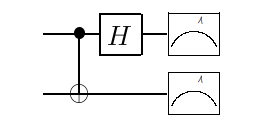
\includegraphics[width=.9\linewidth]{../Quantum_Information_[11/11]/20231127-165019_screenshot.png}
\end{center}
\subsection{MIT MidTerm [2/2]}
\label{sec:orgf9e58d6}
\subsubsection{P2}
\label{sec:orgb13736e}
Entanglement distillation by non-projective measurement. Suppose Alice and Bob
share the two-qubit state \(\left|\psi_{A
B}\right\rangle=(\sqrt{3}|00\rangle+|11\rangle) / 2\). Recall that a quantum
measurement is specified by a set of operators \(\left\{M_0, M_1\right\}\) such
that \(\sum_k M_k^{\dagger} M_k=I\). (a) Give \(a\) and \(b\) such that the quantum
measurement outcome from operator \(M_0=a|0\rangle\langle 0|+b| 1\rangle\langle
1|\) acting on \(\left|\psi_{A B}\right\rangle\) produces the post-measurement
result \((|00\rangle+|11\rangle) / \sqrt{2}\) with probability \(1 / 4\). (15
points) (b) Give an operator \(M_1\) such that \(M_0^{\dagger} M_0+M_1^{\dagger}
M_1=I\). With what probability does the corresponding outcome occur, acting on
\(\left|\psi_{A B}\right\rangle\), and what is the post-measurement result? (10
points)
\subsubsection{P4}
\label{sec:orgb981254}
\begin{enumerate}
\item Qubit tests. Consider the following three-qubit quantum circuit, in which
 \(|\chi\rangle\) and \(|\phi\rangle\) are arbitrary qubits:
\begin{center}
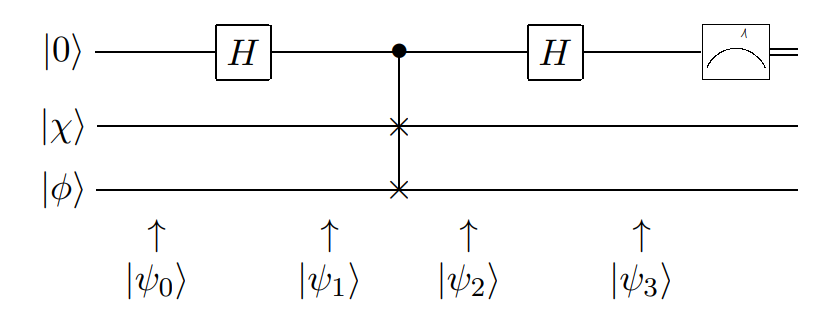
\includegraphics[width=.9\linewidth]{../Quantum_Information_[11/11]/20231127-164944_screenshot.png}
\end{center}
\end{enumerate}

(a) Give the intermediate states of the circuit,
\(\left|\psi_0\right\rangle,\left|\psi_1\right\rangle,\left|\psi_2\right\rangle,\left|\psi_3\right\rangle\).
(4 points each)

(b) If the measurement result is zero (ie the top qubit is \(|0\rangle\) ), what
is the state of the bottom two qubits? (4 points)

(c) If \(|\langle\chi \mid \phi\rangle|=\alpha\), with what probability is the
measurement result zero? (10 points)
\section{Condensed Matter Physics [0/14]}
\label{sec:org7070cff}
\begin{itemize}
\item Provided by Prof. Liu
\end{itemize}
\end{document}